\cotefile{90}
\scanpage{2}
% archive sheet number: 1

\figure{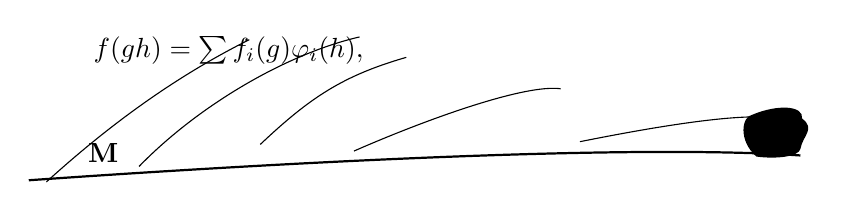
\begin{tikzpicture}[x=.70cm,y=.70cm]
\node[anchor=west] at (1,2.35) {$\deleted{f(gh)=\sum f_i(g)\varphi_i(h),}$};
\node[anchor=west] at (.9,.50) {\uline{$\mathbf M$}};
\draw[thick] (0,0) .. controls (5,.35) and (11,.65) .. (14,.45);
\draw (.32,-.03) .. controls (1.4,.95) and (2.6,1.85) .. (4,2.55);
\draw (2,.25) .. controls (3.1,1.38) and (4.7,2.3) .. (6,2.6);
\draw (4.2,.65) .. controls (5.1,1.5) and (5.7,1.9) .. (6.85,2.23);
\draw (5.9,.53) .. controls (7.2,1.1) and (9,1.75) .. (9.65,1.66);
\draw (10,.7) .. controls (11.2,.94) and (12.5,1.16) .. (13.25,1.15);
\fill (13.2,.43) .. controls (12.87,.72) and (12.93,1.16) .. (13.13,1.19) .. controls (13.58,1.38) and (14.06,1.36) .. (14.03,1.12) .. controls (14.28,.93) and (14.04,.81) .. (14,.57) .. controls (13.97,.43) and (13.57,.38) .. cycle;
\end{tikzpicture}}

\uline{Lemme 1} Soit $A$ un anneau de Dedekind \deleted{\unsure{qui n'est pas un corps}}, $M$ un $A$-module plat. \deleted{Conditions équivalentes} Pour $\forall$ sous-module $N$ de $M$, soit $\widetilde N$ l'image inverse dans $M$ du sous-module de Torsion de $M/N$. Donc $\widetilde N/N$ est un module de torsion.

Cond. équivalentes a) b) c) d)

a) $\forall\, N$ de type fini, $\widetilde N/N$ est de longueur finie, i.e. $\widetilde N$ est de t.f. \margin{$\unsure{\Updownarrow|\Uparrow}$}

b) \deleted{$A$ est un corps,} \inserted{Si $A$ n'est pas un corps,} Il n'existe pas de sous-module de $M$ isomorphe à \deleted{\unsure{$A_p$|$A(p)$}} \inserted{$A(p)=\bigcup_n p^{-n}=\Gamma(S-\{p\},\underline{O}_S)$ $(S=\operatorname{Spec} A)$,} $p$ est un idéal maximal de $A$ \deleted{\unsure{ou} $A$ est un corps.}

c) \deleted{\unsure{Pour tout}} \inserted{Si $A$ n'est pas un corps,} Pour \deleted{$\forall$} \deleted{\unsure{$p$}} idéal maximal $p$ de $A$, $M_p$ ne contient pas de $K$-module isom. à $K$. \margin{$\Updownarrow$}

d) $M=\underset{\longrightarrow}{\lim} M_i$, les $M_i\subset M$ \deleted{de type} fini et ``saturés'', i.e. \inserted{$M_i\unsure{-|\to}M_j$ \unsure{tels|dès} que $M_i$ facteur direct \unsure{de|dans} $M_j$.}

Pour que ces conditions soient \deleted{\unsure{satisfaites}}, il suffit que l'on ait :

e) les formes linéaires sur $M$ séparent, i.e.
\[
\underline M\hookrightarrow A^I \qquad (I\text{ un ensemble})
\]
[condition vérifiée si $M$ contenu \unsure{ds|dans} un libre, \deleted{\unsure{p.}} i.e. $M$ projectif]

C'est aussi nécessaire si $M$ a un ens. dénombrable de générateurs.
\scanpage{3}
% archive sheet number: 2
% Typescript rotated 180 degrees in the scan. Visible spaces left for symbols are retained.

deux cas envisagés dans b), on voit que leur nombre est 1, donc que $B'$ est local. D'autre part, l'hypothèse $X\quad Y$ plat à fibres séparables est héritée par $X4=\deleted{\unsure{X}}\operatorname{Spec}(B')\quad Y'=\operatorname{Spec}(A')$, et les fibres génériques sont isomorphes, ce qui nous permet de remplacer $f:X\quad Y$ par $f':X'\quad Y'$, donc de supposer $Y$ géométriquement unibranche. (Ceci montre d'ailleurs que 19.9.7 est essentiellement contenu dans son corollaire 18.9.11).

Compte tenu de 15.5.6.1. nous sommes ramenés à prouver alors que pour tout $x\quad X$ tel que $f(x)=y$ ne soit pas maximal, $\operatorname{Spec}(\underline O_{X,x})$ n'est pas disconnecté par $x$. Changeant de notations, on est ramené à prouver que lorsque $\dim Y\quad 1$, alors $X$ n'est pas disconnecté par son point fermé $x$. Notons que

\[
\operatorname{prof} B=\operatorname{prof} A+\operatorname{prof} B\otimes_A k
\]

et comme $\operatorname{prof} A\quad 1$, puisque $A$ est intègre de dimension 1, on voit que $\operatorname{prof}(B)\quad 2$ \uline{sauf} si $\operatorname{prof} B\otimes_A k=0$, ce qui équivaut à $\dim B\otimes_A k=0$ puisque par hypothèse $B\otimes_A k$ est séparable sur $k$, donc \deleted{\unsure{intè|inté}} réduit. Or si $\operatorname{prof} B\quad 2$, la conclusion voulue résulte du th. de Hartshorne. \deleted{\unsure{Il reste}}

D'ailleurs, si $A$ est normal, \deleted{\unsure{cette conclusion}} et si $\dim A\quad 2$, on a $\operatorname{prof} A\quad 2$ d'où $\operatorname{prof} B\quad 2$, d'où encore la conclusion voulue. Dans le cas où l'anneau $A$ envisagé dans 18.9.7. est universellement \deleted{\unsure{catégnaire|caténaire},} \inserted{\handwritten{japonais}} \deleted{\unsure{(hypothèse}} \inserted{on peut observer que} \deleted{\unsure{conservée}} dans les réductions précédentes, on peut (sans invoquer $\unsure{0|O}$ 23.2.5 se ramener \deleted{\unsure{directe}} tout de suite au cas $A$ normal (en prenant pour $A'$
le normalisé de $A/\underline p$ dans une extension finie donnée de son corps des fractions), et par suite \deleted{\unsure{en}} l'argument qui précède montre qu'on est réduit au cas où $A$ est de plus de dimension 1, donc spectre d'un anneau de val discrète, et où $B\otimes_A k$ est de dimension 0, donc réduit à un corps, puisqu'il est réduit, ce qui implique aussitôt que $B$ est lui-même un anneau de valuation discrète, donc $X-x$ est réduit à un point et par suite connexe.
\scanpage{4}
% archive sheet number: 3

\uline{Lemme 2} Soit \deleted{$\unsure{B|G}$} $A$ comme dessus, $G$ un $A$-groupe affine, d'algèbre $B$, satisfaisant les conditions ci-dessus. Alors pour tt sous-module de type fini $M$ de $B$, $\exists$ sous-module de type fini $N$ de $B$ tel que $N\supset M$ et tel que

a) $\widetilde N=N$ i.e $N$ saturé -- ce qui implique $N\otimes_A N\hookrightarrow B\otimes_A B$

b) $\Delta N\subset N\otimes N$

\uline{Dém.} Faisons opérer $G\times G$ \deleted{\unsure{sur|à}} sur $B$ par $(g,h)f(s)=f(g^{-1}sh)$. \deleted{Alors \unsure{le|les}} Un sous-module $N$ de $B$ est invariant par $G\times e$ (resp $e\times G$\deleted{\unsure{)}}) \deleted{\unsure{resp}} \unsure{ssi} on a

\[
\Delta N\subset N\otimes B\qquad\text{resp.}\qquad \Delta N\subset B\otimes N.
\]

Notons que \deleted{grâce à la platitude de \unsure{$B|N$}, \unsure{cette}} chacune de ces conditions est stable par passage de $N$ à $\widetilde N$. (\unsure{faire} l'argument).

Donc, la condition d'être invariant par $G\times G$, qui est la conjonction des deux, est aussi stable par passage de $N$ à $\widetilde N$. Or, on sait que $M\subset N$ \inserted{de t.f.} stable par $G\times G$, Par hyp., $\widetilde N$ est encore de t.f., \deleted{\unsure{on a}} et est encore stable \inserted{on peut \unsure{supp.er|supp.} $N=\widetilde N$}.

Mais cela signifie $\Delta\widetilde N\subset(\widetilde N\otimes B)\cap(B\otimes N)=N\otimes N$ cqfd.
\scanpage{5}
% archive sheet number: 4
% Typescript rotated 180 degrees in the scan.

EGA IV 18.9. \qquad (\uline{Rabiots})

L'assertion de connexité faite dans 18.9.1. se généralise de la façon suivante:

\uline{Théorème} 18.9.7. Soit $A\quad B$ un homomorphisme local d'anneaux locaux noethériens, et supposons a) \inserted{$f:$} $\operatorname{Spec}(B)=X\quad\operatorname{Spec}(A)=Y$ est plat à fibres séparables, et b) $A$ est géométriquement unibranche, ou $A$ est unibranche et $k(B)$ une extension primaire de $k(A)$. Alors la fibres générique de $X$ sur $Y$ est connexe, et pour toute partie fermée $\unsure{S|\mathbb S|Z}$ de $Y$ distincte de $Y$, \deleted{$\unsure{f^{-1}|X-f^{-1}}$} et tout fermé $T$ de $X$ contenu dans $f^{-1}(S)$, $X-T$ est connexe.

Signalo\deleted{\unsure{p}}ns tout de\deleted{\unsure{s}} suite les corollaires suivants:

\uline{Corollaire} 18.9.8. Supposons qu'on ait a) ci-dessus, et b') $A$ est strictement local, ou $A$ est local hensélien et $k(B)$ est une extension primaire de $k(A)$. Alors \uline{toutes} les fibres de $X$ sur $Y$ sont \uline{géométriquement connexes}.

En effet, soit $A\quad A'$ un homomorphisme local, avec $A'$ fini sur $A$, et soit $B'=B\otimes_A A'$, alors on constate aussitôt que les hypothèses faites sont encore vérifiées pour $A'\quad B'$. Ceci nous ramène, comme d'habitude, au cas où $A$ est intègre, et à vérifier que dans ce cas, la fibre générique de $f:X\quad Y$ est connexe. Mais nous sommes alors sous les conditions du théorème qui précède.

\uline{Corollaire} 18.9.9. Soit $A$ un anneau local noethérien hénsélien, \deleted{\unsure{à fi}} universellement caténaire (i.e. réf \quad à fibres formelles séparables). Alors les fibres formelles de $A$, i.e. les fibres de $\operatorname{Spec}(\hat{\hat A})\quad\operatorname{Spec}(A)$, sont \inserted{\handwritten{géom}} connexes.

C'est en effet un cas particulier de 18.9.8. (l'extension résiduelle $k(\widehat{\unsure{\mathbb A|A|B}})$ sur $k(A)$ est ici triviale, à fortiori primaire).
\scanpage{6}
% archive sheet number: 5
% Vertical emphasis stroke at the left of the first corollary.

\margin{\rule{.04em}{1.5em}}\uline{Corollaire} Si \inserted{de plus} $G$ est de t.f. sur $A$, alors $G$ admet une représentation linéaire fidèle.

Il existe $N$ tel que a) $N$ engendre l'algèbre $B$, b) $\widetilde N=N$, c) $\Delta N\subset N\otimes \unsure{B|N}$.
\deleted{\unsure{Le}} Alors \deleted{\illegible{1}} \unsure{tt|un} $\mathrm p^{\mathrm t}$ de $G$ à valeurs dans $A'/A$ qui opère \unsure{trivmt|trivemt|trivialement} sur $N'$, opère \unsure{trivialmt|trivialement} sur $B'$, \deleted{\unsure{donc c'est}} donc est \deleted{\unsure{un}} l'unité. Donc la repr. est fidèle.

\uline{Corollaire} Si $A$ est un corps $k$, alors, tt groupe affine \deleted{\unsure{est}} $G$ sur $k$ est lim. \deleted{\unsure{inductive}} projective d'un syst. projectif strict (\unsure{morph.} de transition des morphismes \unsure{fid|fid.} plats) de groupes affines \uline{de t.f.}.
\scanpage{7}
% archive sheet number: 6
\mspage{\handwritten{-3-}}

\uline{Corollaire} (18.9.5) .- \uline{Sous les hypothèses de} (18.9.4) , \uline{le foncteur}

\[
Z\handwritten{\rightsquigarrow} Z\handwritten{\otimes}_A A'\tag*{(18.9.5.1)}
\]

\uline{de la catégorie des préschémas étales sur} $X$ , \uline{dans celle des préschémas étales sur} $X'$ , \uline{est pleinement fidèle} .

Soient $Z_1,Z_2$ deux préschémas étales sur $X$ , et\deleted{\unsure{X}} posons $Z_{\unsure{i|1}}'=Z_i\handwritten{\otimes}_A A'$ $(i=1,2)$ \,; \deleted{\illegible{2}} il s'agit de prouver que tout $X'$-morphisme $Z_1'\handwritten{\longrightarrow} Z_2'$ provient , par changement de base , d'un\inserted{$X$-}morphisme unique $Z_1\handwritten{\longrightarrow} Z_2$ .
\margin{\handwritten{\tikz{\draw (0,0)--(.55,.05) (0,-.11)--(0,.12) (.55,-.06)--(.55,.17);}}}Supposons d'abord que \deleted{$Z_1$ et} $Z_2$ soi\deleted{en}t \uline{séparé\deleted{s}} sur $X$ ; alors, comme $\operatorname{Hom}_X(Z_1,Z_2)$ s'identifie à \deleted{\illegible{1}} $\handwritten{\Gamma}(Z_1\handwritten{\times}_X Z_2/Z_1)$ , et que $Z_1\handwritten{\times}_X\unsure{\mathbb Z|Z}_2$ est étale et séparé sur $Z_1$ , $\operatorname{Hom}_X(Z_1,Z_2)$ s'identifie fonctoriellement, en vertu de (17.9.3) , à l'ensemble des parties ouvertes et fermées $U$ de $Z_1\handwritten{\times}_X Z_2$ telles que la restriction à $U$ de la projection $p:\ Z_1\handwritten{\times}_X Z_2\handwritten{\longrightarrow} Z_1$ soit un morphisme surjectif et radiciel . L'assertion résulte donc dans le cas considéré de (18.9.4) et de ce que $Z_1'\handwritten{\times}_{X'} Z_2'={}= (Z_1\handwritten{\times}_X Z_2)\handwritten{\otimes}_A A'$ .

Passons au cas général : il suffira de prouver que le graphe $\handwritten{\Gamma}'$ d'un $X'$-morphisme $Z_1'\handwritten{\longrightarrow} Z_2'$ \inserted{qui est \uline{ouvert} (17.9.3) \handwritten{dans $Z_1'\times_{X'} Z_2'$}} est de la forme $\handwritten{\Gamma}\handwritten{\otimes}_A A'$ , où $\handwritten{\Gamma}$ est \deleted{\unsure{un ouvert}} induit sur une partie \uline{ouverte} de $Z=Z_1\handwritten{\times}_X Z_2$ . En effet , la restriction à $\handwritten{\Gamma}$ de la projection $p:\ Z\handwritten{\longrightarrow} Z_1$ est alors un \uline{isomorphisme} , car par changement de base \inserted{$A\handwritten{\longrightarrow} A'$} cette restriction devient l'isomorphisme restriction à $\handwritten{\Gamma}'$ de la projection $p':\ Z'\handwritten{\longrightarrow} Z_1'$ (avec $Z'=Z\handwritten{\otimes}_A A'$) , et \margin{\handwritten{\tikz{\draw (0,0) .. controls (.32,.20) and (.50,.03) .. (.54,.21);}}}il suffit d'appliquer (2.7.1,(viii)) ; la conclusion résulte donc \inserted{\handwritten{alors}} de la caractérisation des graphes de morphismes (\uline{I},5.3) .

Si $q:\ Z'\handwritten{\longrightarrow} Z$ est la projection canonique , pour prouver que $\handwritten{\Gamma}'$ est de la forme \deleted{\illegible{1}} $q^{-1}(\handwritten{\Gamma})$ , où $\handwritten{\underline{\Gamma}}$ est ouvert \inserted{dans $Z$} , il suffit , puisque $q$ est un morphisme \inserted{fidèlement} plat \inserted{et quasi-compact} , de prouver \deleted{\unsure{que}} qu'il existe un ensemble $U\handwritten{\subset} Z$ tel que $\handwritten{\Gamma}'=q^{-1}(\unsure{U|V})$ (2.3.12) . Posons $Z''=Z'\handwritten{\times}_Z Z'=Z\handwritten{\times}_X X''$ , où $X''=X'\handwritten{\times}_X X'$ , et soient $q_1:\ Z''\handwritten{\longrightarrow} Z'$ , $q_2:\ Z''\handwritten{\longrightarrow} Z'$ les projections canoniques . Appli-
\scanpage{8}
% archive sheet number: 7

\uline{Prop} $A$ anneau, $G$ groupe affine sur $A$, d'algèbre $B$. On suppose que en tant que $A$-module, on a $B=\underset{\longrightarrow}{\lim} B_i$, où $B_i\subset B$ sont tels que

a) $B/B_i$ est plat /$A$, \deleted{b)} donc \deleted{$\unsure{\Delta}$} $B_i\otimes B_i\subset B\otimes B$, et b) $\Delta B_i\subset B_i\otimes B_i$.

\deleted{\unsure{Soit}} c) les $B_i$ sont projectifs de t.f.

\deleted{Alors} Pour $i$ fixé, utilisant a), on voit que pour tt $A$-module $E$, $B_i\otimes E\subset B\otimes E$.

Si $G$ opère sur $E$, disons que $E$ est $i$-admissible si $\delta:E\unsure{\mathrel{-}|\to} B\otimes E$ se factorise par $B_i\otimes E$, donc est défini par

\[
\delta_i:E\mathrel{-} B_i\otimes E.
\]

Alors la catégorie des $A$-$G$-modules \inserted{de t.f.} est la limite inductive, pour $i$ variable, des ss-catégories $\unsure{C_i|\mathcal C_i}(\deleted{\unsure{A_i|A}}\unsure{B|A|G})_f$ des $A$-$G$-modules admissibles \inserted{de t.f.}. D'autre part, utilisant b) et c), et introduisant $U_i=\check B_i$, on trouve que $U_i$ est une algèbre ass. unitaire
\deleted{\unsure{(une}} \deleted{\unsure{non, si} $1\in \unsure{G|B}$ $i$ assez grand pour que $\unsure{\varepsilon}(B_i)=A$,\unsure{\}|]}} \deleted{\unsure{p. ex. pour} $1\in \unsure{B_i|E_i}$\unsure{]}} Alors, les \deleted{\unsure{catégorie|catégories} $C_i$} $U_i$
\scanpage{9}
% archive sheet number: 8
\mspage{- IV-\handwritten{965} -}
% Two long oblique strokes cancel the lower corollary; a wavy stroke also crosses the remark.

\uline{Corollaire} (18.9.4) .- \uline{Soit} $A$ \uline{un anneau local noethérien , hensélien et dont les fibres formelles sont géométriquement normales} \deleted{\illegible{1}} (par exemple un anneau local noethérien hensélien et \uline{excellent}) , \uline{et posons} $A'=\hat A$ . \uline{Soient} $X$ \uline{un} $A$-\uline{préschéma} , $X'=X\handwritten{\otimes}_A A'$ , $g:\ X'\handwritten{\to} X$ \uline{la projection canonique . Alors l'application} $U\handwritten{\rightsquigarrow} g^{-1}(U)$ \uline{est une bijection de l'ensemble des parties à la fois ouvertes et fermées de} $X$ \uline{sur l'ensemble des parties à la fois ouvertes et fermées de} $X'$ .

Comme $g$ est un morphisme \deleted{\unsure{très|f}} fidèlement plat et quasi-compact , on sait (2.3.12) que la topologie de $X$ est \uline{quotient} de celle de $X'$ par la relation d'équivalence définie par $f$ . Tout revient donc à voir \deleted{\unsure{que}} qu'une partie ouverte et fermée $U'$ de $X'$ est \uline{saturée} pour cette relation . Or , comme le morphisme $\operatorname{Spec}(A')\handwritten{\to}\operatorname{Spec}(A)$ \deleted{\unsure{est}} a ses fibres géométriquement connexes (18.9.1) , les fibres de $g$ sont \uline{connexes} , d'où aussitôt notre assertion .

En particulier , si $X$ est localement connexe (ce qui sera le cas si $X$ est localement noethérien) , alors , pour toute \deleted{\unsure{partie connexe}} composante connexe $U$ de $X$ \handwritten{(} qui est ouverte et fermée dans $X$ \handwritten{),} $g^{-1}(U)$ est connexe (Bourbaki, \uline{Top.gén.},chap.I,$3^{\mathrm e}$ éd.,\S\ 11,n$^{\mathrm o}$3 ,\handwritten{prop 7} ) . Si l'on désigne par $\handwritten{\pi}_0(X)$ l'ensemble des composantes connexes de $X$ , , l'application $\handwritten{\pi}_0(X')\handwritten{\to}\handwritten{\pi}_0(X)$ déduite canoniquement de $g$ est donc \uline{bijective} .

\deleted{\uline{Corollaire} (18.9.5) .- \uline{Sous les hypothèses de} (18.9.4) , \uline{le foncteur}}

% slanted
\margin{\handwritten{``séparés'' inutile !}}

\deleted{\[
Z\handwritten{\rightsquigarrow} Z\handwritten{\otimes}_A A'\tag*{(18.9.5.1)}
\]}

\deleted{\uline{de la catégorie des} \deleted{$X$-}\inserted{\handwritten{pré}}\uline{schémas étales} \deleted{\handwritten{(resp. étales et finis)}} \inserted{\handwritten{et séparés}} \uline{sur} $X$ \uline{dans celle des} \deleted{\illegible{2}} \deleted{\unsure{$X'$-|$X$-}}\inserted{\handwritten{pré}}\uline{schémas étales} \deleted{\handwritten{(resp. étales et finis)}} \inserted{\handwritten{et séparés}} \uline{sur} $X'$ , \uline{est pleinement fidèle} .}

% slanted
\margin{\handwritten{la \unsure{var.|vers.|vrai} n'apporte rien ; $X$-schéma risque d'induire en erreur ---}}

\deleted{En effet , si $Z_1,Z_2$ sont deux $X$-schémas étales sur $X$ , $\operatorname{Hom}_X(Z_1,Z_2)$ s'identifie à $\handwritten{\Gamma}(Z_1\handwritten{\times}_X Z_2/Z_1)$ , et $Z_1\handwritten{\times}_X Z_2$ est étale et séparé sur $Z_1$ , donc finalement (17.9.3) , $\operatorname{Hom}_X(Z_1,Z_2)$ s'identifie fonctoriellement à l'ensemble des parties ouvertes et fermées $U$ de $Z_1\handwritten{\times}_X Z_2$ telles que la restriction de la projection $p:\ Z_1\handwritten{\times}_X Z_2\handwritten{\to} Z_1$ à $U$ soit un morphisme surjectif et radiciel . L\deleted{a}\inserted{e} corollaire résulte donc aussitôt de (18.9.4) et du fait que , si $Z_i'=Z_i\handwritten{\otimes}_A A'$ \deleted{\illegible{1}} $(i=1,2)$ , on a $Z_1'\handwritten{\times}_{X'} Z_2'=(Z_1\handwritten{\times}_X Z_2)\handwritten{\otimes}_A A'$ .}

\deleted{\uline{Remarques} (18.9.6) .- \deleted{\unsure{i)} Dans tous les cas connus} \inserted{\handwritten{Il est possible que si le corps résiduel de $A$ est de car. nulle,}} le foncteur (18.9.5.1) \deleted{\unsure{est}} \inserted{\handwritten{induit}}}
\scanpage{10}
% archive sheet number: 9
% Vertical emphasis stroke at left of the corollary.

forment un syst. projectif \inserted{strict} d'algèbres sur $A$. $\unsure{C_i|\mathcal C_i}(\unsure{G|B})_f$ est équivalente \unsure{canoniqt|canoniqmt|canoniquement} à la catégorie des $U_i$-modules \inserted{de t.f.}. Et les \deleted{foncteurs} \unsure{transitions|transition} \deleted{\unsure{entre}} les $C_i(G)$ sont isomorphes aux \deleted{\unsure{aux}} \deleted{foncteurs} \uline{restriction des scalaires}

\margin{\rule{.04em}{2.6em}}\uline{Corollaire} Sous les conditions précédentes, tt module \inserted{de t.f. $E$} d'une représentation de $G$ est quotient d'un module \inserted{\uline{projectif}} de t.f. où $G$ opère.

\uline{Prop} Soit $G$ gpe affine plat sur $A$ anneau de Dedekind, d'algèbre $B$ satisfaisant aux conditions du lemme 1 (\unsure{NB.} si $G$ est de t.f. cela signifie que pour tte composante irréd. de $G$, \uline{ttes} ses fibres sont non vides).

Soit \deleted{\unsure{$A'$ une $A$-algèbre}} $\unsure{S|S'}$ un schéma sur $S$, tel que sur $S$, tt module qu. coh. de t.f. \deleted{admette une \unsure{résolut.}} \inserted{soit isomorphe} à un quotient d'un module loc. libre de t.f.

\deleted{Alors} (p. ex. $S$ admet \unsure{modules|module} inv. \unsure{amples|ample}, ou $S$ noeth. régulier). Alors tt
\scanpage{11}
% archive sheet number: 10
\mspage{- IV-\handwritten{964} -}

\uline{Pour que} $A$ \uline{soit unibranche} (resp. \uline{géométriquement unibranche) , il faut et il suffit que} $\operatorname{Spec}(A)$ \uline{soit irréductible} .

\uline{Proposition} (18.8.1\deleted{3}\handwritten{\unsure{6|5}}) .- \uline{Soit} $A$ \uline{un anneau local noethérien . Si} $A$ \uline{est universellement caténaire , il en est de même de} $ {}^{\mathrm{hs}}A$ .

La démonstration est la même que celle de (18.7.5) .

\uline{18.9. Fibres formelles des anneaux noethériens henséliens} .

\uline{Théorème} (18.9.1) .- \uline{Soit $A$ un anneau local noethérien hensélien , dont les fibres formelles sont géométriquement normales . Alors les fibres formelles de} $A$ \uline{sont géométriquement intègres} (donc \uline{géométriquement connexes}) ,

Les deux assertions de l'énoncé sont en fait équivalentes,un préschéma \inserted{localement noethérien} connexe et normal étant intègre . Comme toute $A$-algèbre intègre finie est un anneau local hensélien (18.5.9 et 18.5.10) , il résulte de (7.3.16.2) que l'on est ramené à prouver que si l'on suppose de plus $A$ \uline{intègre} , alors la fibre du morphisme $\operatorname{Spec}(\hat A)\handwritten{\to}\operatorname{Spec}(A)$ au point générique de $\operatorname{Spec}(A)$ est \uline{intègre} , ce qui résulte du

\uline{Corollaire} (18.9.2) .- \uline{Soit} $A$ \uline{un anneau local noethérien hensélien intègre, dont les fibres formelles sont géométriquement normales . Alors} $\hat A$ \uline{est intè}\deleted{\unsure{géométr.|intègres}}\uline{gre} .

En effet , il résulte de (18.8.12) que $A$ est unibranche , \handwritten{d}onc \deleted{\illegible{2}} le théorème résulte de l'hypothèse faite sur les fibres formelles de $A$ et de (7.6.3) .

\uline{Corollaire} (18.\deleted{\unsure{8}}\handwritten{9}.3) .- \uline{Sous les hypothèses de} (18.9.2) , \uline{le corps des fractions} $L$ \uline{de} $\hat A$ \uline{est une extension séparable du corps des fractions} $K$ \uline{de} $A$ , \uline{e\handwritten{t}} $K$ \uline{est algébriquement fermé dans} $L$ .

\deleted{\illegible{2}} \deleted{La première assertion} \inserted{\handwritten{Cela}} résulte de ce que la fibre du \unsure{morphisme|mbrphisme} $\operatorname{Spec}(\hat A)\handwritten{\to}\handwritten{\to}\operatorname{Spec}(A)$ au point générique de $\operatorname{Spec}(A)$ est géométriquement \deleted{\unsure{intègre}} intègre et de (\handwritten{4.3.2} ) \handwritten{et (4.3.5).}
\scanpage{12}
% archive sheet number: 11

$G_S$-module \deleted{\unsure{admet}} qu. coh. de t.f. est quotient d'un \unsure{idem}, qui est de plus \uline{loc. libre}.
\scanpage{13}
% archive sheet number: 12
\mspage{- IV-\handwritten{\unsure{963|96}} -}

\uline{briques séparables de} $\handwritten{\kappa}(\underline p)$ (ce qui entraîne que les fibres du \unsure{morphisme} canon\handwritten{i}que $\operatorname{Spec}({}^{\mathrm{hs}}A)\handwritten{\to}\operatorname{Spec}(A)$ sont \uline{géométriquement régulières}) .

\uline{Corollaire} (18.8.\deleted{9}\handwritten{12}) .- \uline{Soit} $A$ \uline{un anneau local noethérien . Pour que} $ {}^{\mathrm{hs}}A$ \uline{possède une des propriétés suivantes}\deleted{\unsure{,}} :

a) \uline{être un anneau de Cohen-Macaulay} ;

b) \uline{vérifier la condition} $(S_n)$ ;

c) \uline{être régulier} ;

d) \uline{vérifier la condition} $(R_n)$ ; \margin{\handwritten{\tikz{\draw (0,0) .. controls (.05,-.4) and (.07,-.5) .. (.18,-.8); \draw (-.65,-.27) .. controls (-.65,-1) and (-.31,-.81) .. (.18,-.8); \draw (-.65,-1.25) .. controls (-.54,-.90) and (-.22,-.78) .. (.18,-.8);} \unsure{11|''}\,$\vert$}}

\uline{il faut et il suffit que $A$ possède cette même propriété} .

\uline{Corollaire} (18.8.1\deleted{0}\handwritten{3}) .- \uline{Soit} $A$ \uline{un anneau semi-local noethérien . Pour qu'un idéal premier} $\underline p$ \uline{de} $ {}^{\mathrm{hs}}A$ \uline{appartienne à} $\operatorname{Ass}({}^{\mathrm{hs}}A)$ , \uline{il faut et il suffit que} $\underline p\handwritten{\in} A$ \uline{appartienne à} $\operatorname{Ass}(A)$ .

Les démonstrations sont les mêmes que celles de (18.6.9),(18.6.10) et (18.6.11) respectivement .

\uline{Proposition} (18.8.1\deleted{1}\handwritten{4}) .- \uline{Soit} $A$ \uline{un anneau local ; les propriétés suivantes sont équivalentes} :

a) $A$ \uline{est géométriquement unibranche} (resp. \uline{réduit et géométriquement unibranche}) .

b) \uline{Pour toute} $A$-\uline{algèbre locale essentiellement étale} $A'$ , $\operatorname{Spec}(A')$ \uline{est irréductible} (resp. \uline{intègre}) .

c) $\operatorname{Spec}({}^{\mathrm{hs}}A)$ \uline{est irréductible} (resp. \uline{intègre}) .

On se ramène comme dans (18.6.1\handwritten{2}) au cas où $A$ est réduit \handwritten{[}, \uwave{en utilisant (18.8.7.1) ,}\handwritten{]}\margin{\handwritten{\unsure{!|?}}} et l'équivalence de b) et c) se prouve comme dans (18.6.1\handwritten{2}) ; i\handwritten{l} en est de même du fait que a) entraîne c) , en tenant compte de (18.8.7.1) et de la définition d'un anneau local intègre géométriquement unibranche . Enfi\handwritten{n} pour démontrer que c) entraîne a) , gardons les mêmes notations que dans (18.6.1\handwritten{2}) ; il s'agit encore de voir que $ {}^{\mathrm{hs}}B$ est intègre . Mais , par (18.8.7) , $ {}^{\mathrm{hs}}B$ est un anneau local de l'anneau semi-local $B\handwritten{\otimes}_A({}^{\mathrm{hs}}A)$ , qui s'identifie encore par platitude à un sous-anneau du corps $L$ , donc est intègre ; il en est par suite de même de $ {}^{\mathrm{hs}}B$, \handwritten{\unsure{/}}ce qui achève la démonstration .

\deleted{\unsure{Proposition}}\inserted{Corollaire} (18.8.1\deleted{2}\handwritten{5}) .- \uline{Soit} $A$ \uline{un anneau \inserted{local} hensélien} (resp\handwritten{.} \uline{strictement local}\handwritten{)}
